\chapter{Implementation}

\section{Aufbau}
Die Implementation besteht aus einem CMS in welchem der Content von einer oder mehreren Apps verwaltet werden kann. Die Inhalte werden in einer Datenbank gespeichert. Eine iPhone App kann sich dann die Inhalte aus der Datenbank herunterladen und darstellen, bzw. verarbeiten.

\section{Datenstruktur}
Um eine gr�sstm�gliche Flexibilit�t zu gew�hrleisten wird die Datenstruktur nicht vorgeschrieben, sondern kann den Bed�rfnissen angepasst erstellt werden.

\begin{figure}[H]
	\centering
	\includegraphics[scale=0.8]{graphics/entityModel.png}
	\caption{\textbf{Entity Model} }
	\label{entityModel}
\end{figure}

In \autoref{entityModel} ist das Entit�tenmodell zu sehen auf welchem die Datenbank beruht. 

\subsection{Field\_types}
\emph{field\_types} k�nnen beliebig defniert werden. Es kann sich dabei um ein Attribut handeln, welches einen Status beschreiben soll, oder um eine Beschreibung eines Elements. Typische \emph{field\_types} sind z.B: text, url, color. Wichtig ist, dass ein \emph{field\_type} nicht einem Datentyp entsprechen muss. \\


\subsection{Templates}
Die \emph{Templates} sind das Herzst�ck der Datenstruktur. Es handelt sich dabei um eine Art Schablone, welche die Struktur f�r ein beliebiges Element vorgibt. Ein \emph{Template} kann entweder aus beliebig vielen \emph{Field\_types} bestehen (einfaches Template) oder aus beliebig vielen anderen \emph{Templates} und \emph{Field\_types} (Composite Template). \\
\\
Als Beispiel daf�r kann man sich ein Buch vorstellen, welches aus einem Titel und mehreren Kapiteln besteht. Titel und Kapitel w�ren \emph{Templates} welche aus dem \emph{Template} text bestehen und das \emph{Template} Buch w�rde aus den \emph{Templates} Titel und Kapitel bestehen.

\subsection{Articles}
Jeder \emph{Article} beruht auf einem \emph{Template}. Ein \emph{Article} ist die Umsetzung eines \emph{Templates} und entspricht einer dargestellten Seite in der App. Das \emph{Template} gibt die Struktur vor und die Daten werden entsprechend dieser Vorgabe als json-String abgelegt.

Die Mobile App interpretiert dann diesen json-String anhand der durch das Template vorgegebenen Struktur und stellt die Seite dar.

\section{Datenbank}
Als Datenbank haben wir uns f�r SQLite entschieden, da diese von allen verbreiteten Smartphone Systemen sehr gut unterst�tzt wird. \\
\\
Um die oben beschriebene Struktur in einer relationalen Datenbank abzubilden wird die Datenbank wie folgt aufgebaut:

\begin{figure}[H]
	\centering
	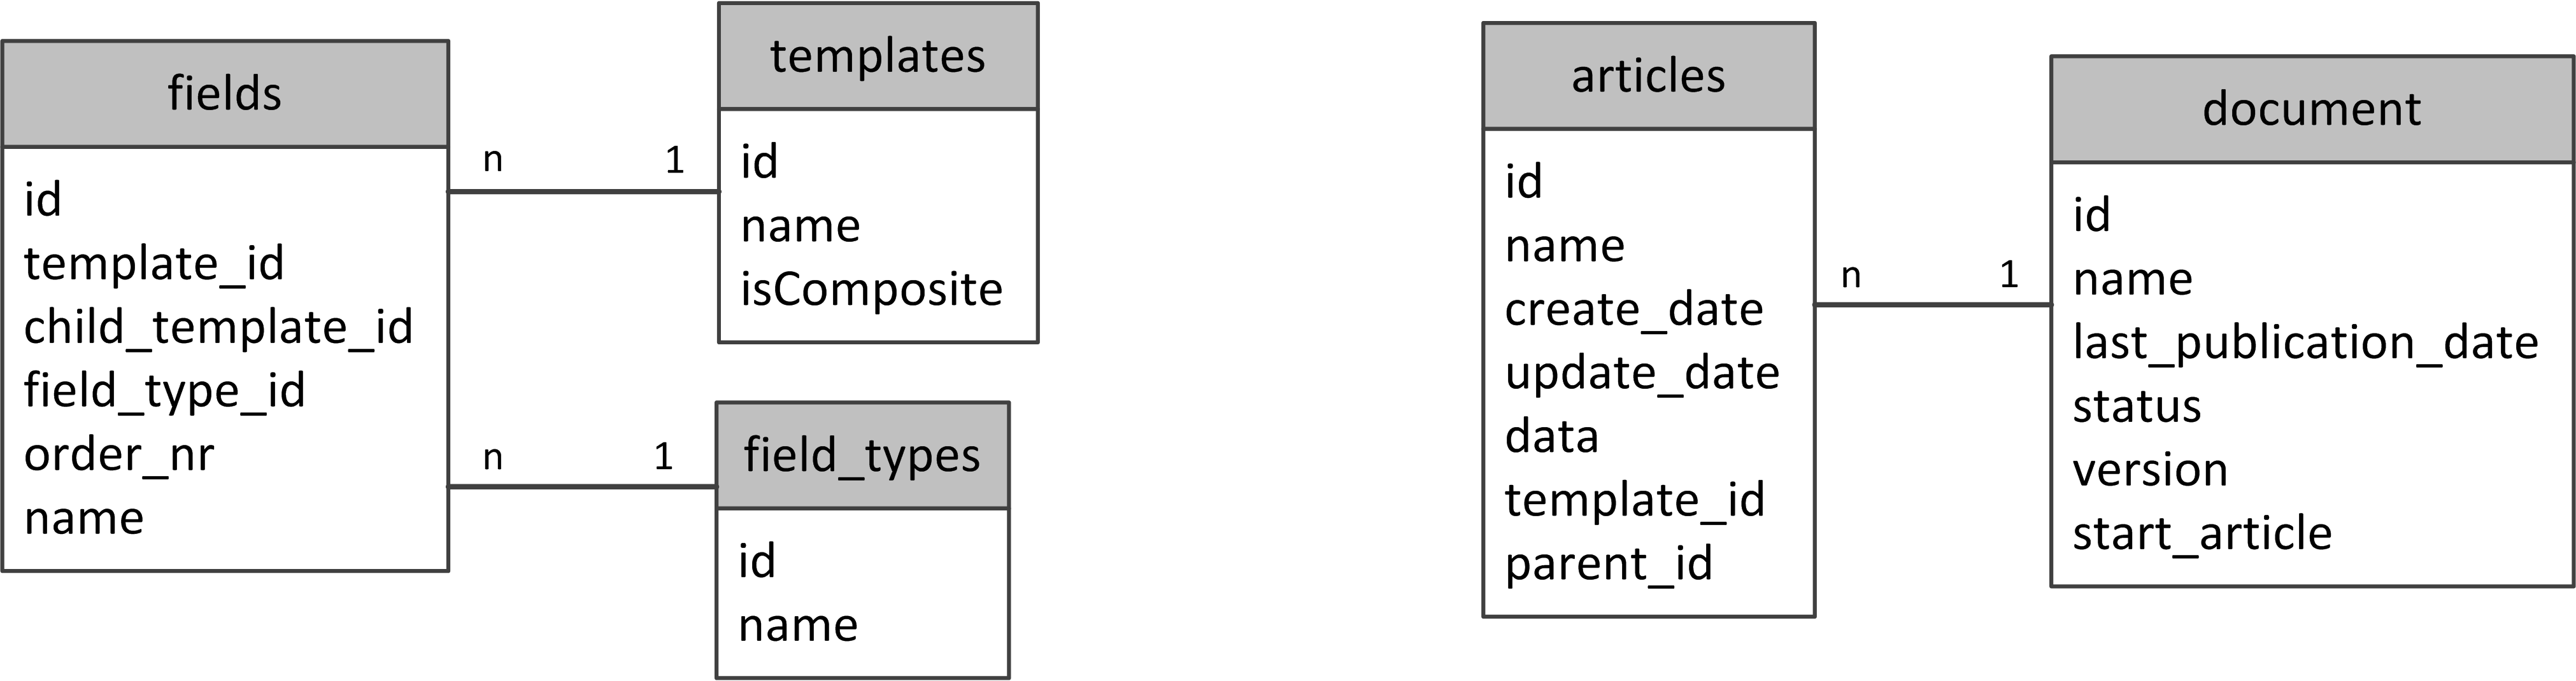
\includegraphics[scale=0.8]{graphics/db.png}
	\caption{\textbf{Database Model} }
	\label{dbModel}
\end{figure}

Die Zwischentabelle \emph{fields} wird ben�tigt um die Verschachtelung der \emph{Templates} und \emph{Field\_Types} zu erm�glichen. Jeder \emph{Article} ist einem  \emph{document} zugeordnet. Im \emph{document} wird der Start Artikel, Status und die Version der Daten festgehalten. Werden mehrere Apps in einer Datenbank verwaltet werden mehrere \emph{documents} erstellt.


\section{CMS}
Das CMS haben wir mit PHP entwickelt. Um die Benutzeroberfl�che schneller und benutzerfreundlicher gestalten zu k�nnen haben wir das Framework Optimus Dashboard genutzt. Das CMS ist in die Bereiche Dashboard, Documents, Articles, Templates und Assets unterteilt.

\subsection{Dashboard}
Dieser Bereich wird noch nicht gebraucht. Das Ziel ist es hier generelle Informationen anzuzeigen

\subsection{Documents}
Hier werden einzelne Documents (Apps) erstellt und verwaltet. Es kann der Startartikel f�r die App angegeben werden sowie die Version der Daten und der Status der App angepasst werden.

\subsection{Articles}
Dies ist der wichtigste Teil f�r die Bereitstellung von Inhalten. Hier werden die Artikel (Seiten der App) erstellt und bearbeitet. 

Um die Daten m�glichst einfach einzugeben, muss das CMS pro \emph{field\_type} eine ensprechende Eingabemaske anbieten (f�r \emph{text} ein Textfeld, f�r \emph{color} ein Color Picker, etc.).


\subsection{Templates}
Die f�r die Einrichtung wichtigen Templates k�nnen hier zusammengestellt werden. Dazu erlaubt das CMS die ben�tigten Felder zu verkn�pfen und zu gruppieren.

\subsection{Assets}
S�mtliche Resourcen wie Bilder, Videos, etc. k�nnen hier verwaltet werden.

\section{App}
Das Ziel ist, dass die App generisch ist, und grunds�tzlich keine Styles oder Bilder enth�lt. Jedes im CMS vorhandene Template sollte verarbeitet werden k�nnen. Dazu muss f�r iOS ein View Controller und f�r Android eine Activity implementiert sein. Bei anderen Systemen muss ebenfalls die Logik implementiert werden dass die m�glichen Templates verarbeitet und dargestellt werden. Je mehr Templates definiert sind und von der App unterst�tzt werden, desto mehr M�glichkeiten bieten sich an.

\subsection{Auf neue Inhalte �berpr�fen}

\begin{figure}[H]
	\centering
	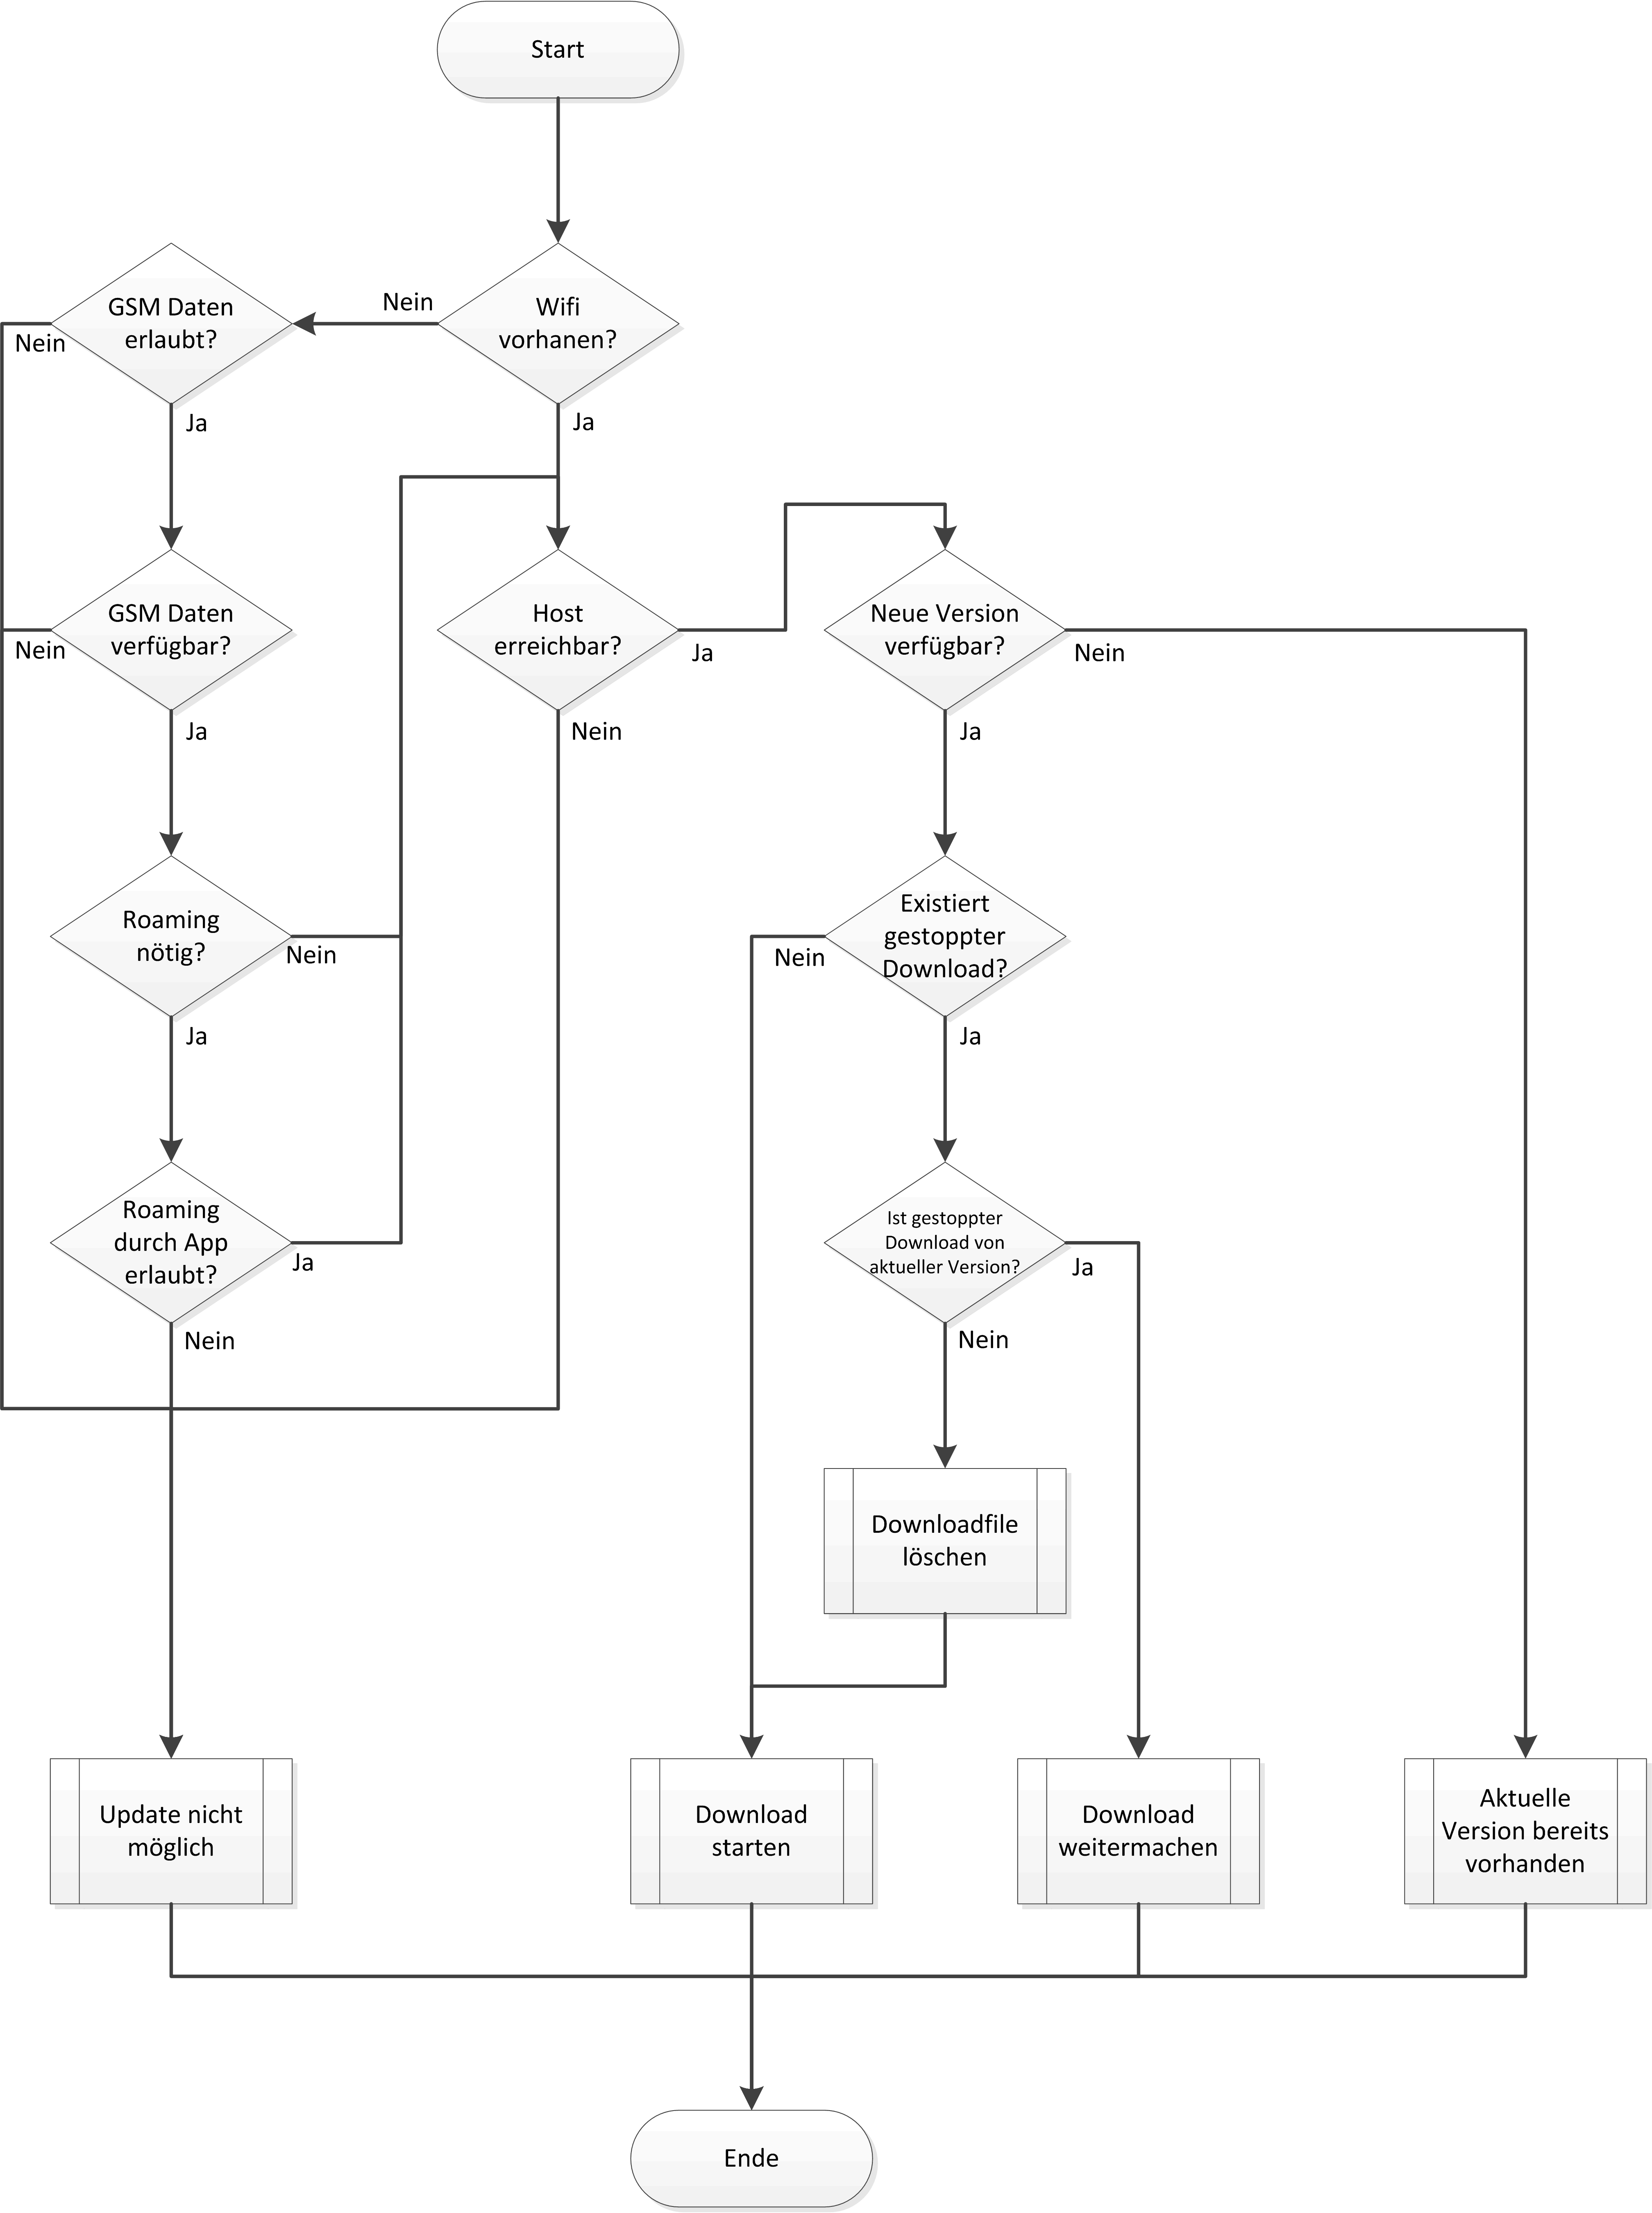
\includegraphics[scale=0.6]{graphics/Netzwerk-Check-FlowChart.png}
	\caption{\textbf{Ablaufdiagramm - Daten Update} }
	\label{NWCheck}
\end{figure}

\autoref{NWCheck} zeigt das Vorgehen der App zur Pr�fung ob neue Daten vorhanden sind. Wichtig ist die �berpr�fung ob Wifi vorhanden ist, bzw ob GSM Daten erlaubt sind. GSM steht hier stellvertretend f�r alle Mobiltelefonnetze. Da eine Datenverbindung �ber ein Mobiltelefonnetz mit Kosten verbunden sein kann (speziell Roaming-Geb�hren), fragt die App in diesem Fall nach, ob eine Verbindung gemacht werden darf. \\

\subsection{Interpretation von Artikeln}
Um ein Artikel darzustellen, analysiert die App den json-String, welcher im Datenfeld des Artikels hinterlegt ist. Anhand des Templates weiss die App wie der json-String zerlegt werden muss und die entsprechenden Elemente darzustellen sind.

\begin{figure}[H]
	\centering
	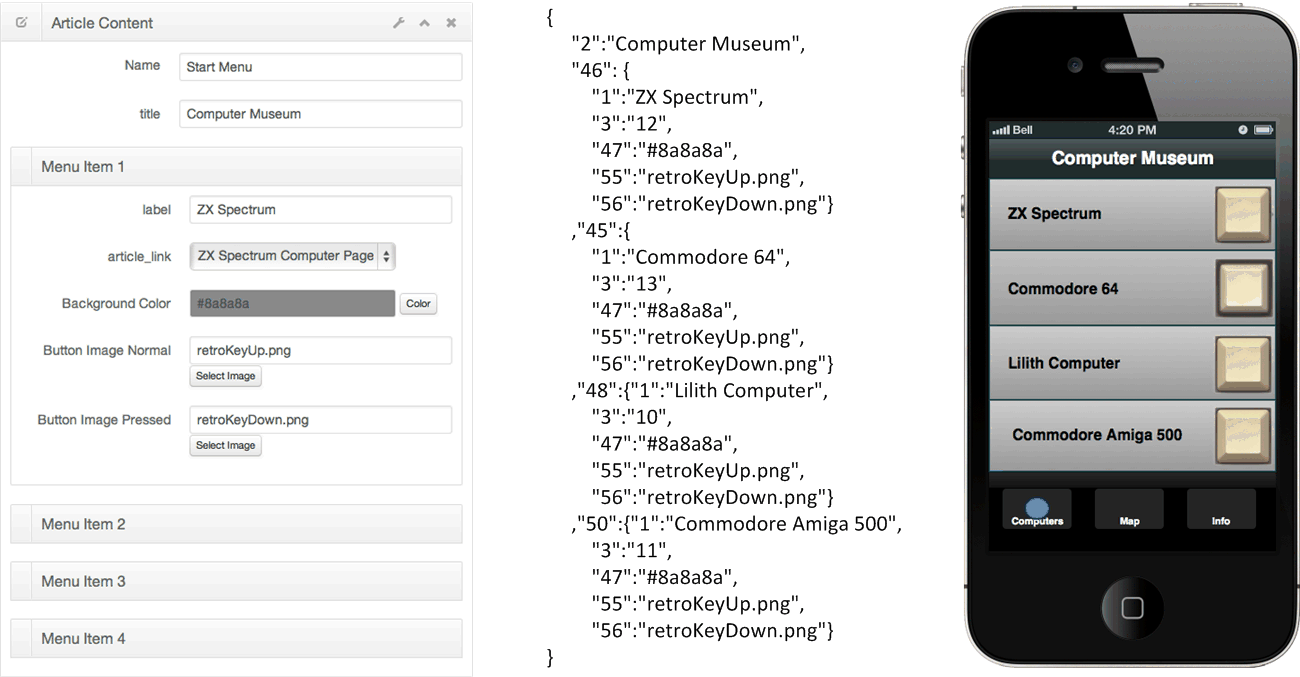
\includegraphics[scale=0.6]{graphics/jsonBsp.png}
	\caption{\textbf{Interpretation des json-Sting}}
	\label{jsonBsp}
\end{figure}

In \autoref{jsonBsp} sehen wir die schematische Darstellung des Templates im CMS, den json-String welcher das Template umsetzt und die Darstellung in der App.
